In the each of the following exercises, find the coordinates of the focus, vertex, eccentricity, axis of the conic section, the equation of the directrix and the length of the latus rectum.
\begin{enumerate}[label=\thesubsection.\arabic*,ref=\thesubsection.\theenumi]
\item $y^2=12x$ 
\label{chapters/11/11/2/1}
\\
\solution
See \tabref{tab:rot-conic-params-sol}
and 
\figref{fig:chapters/11/11/2/4/Fig1}.
\begin{figure}[H]
	\begin{center} 
	    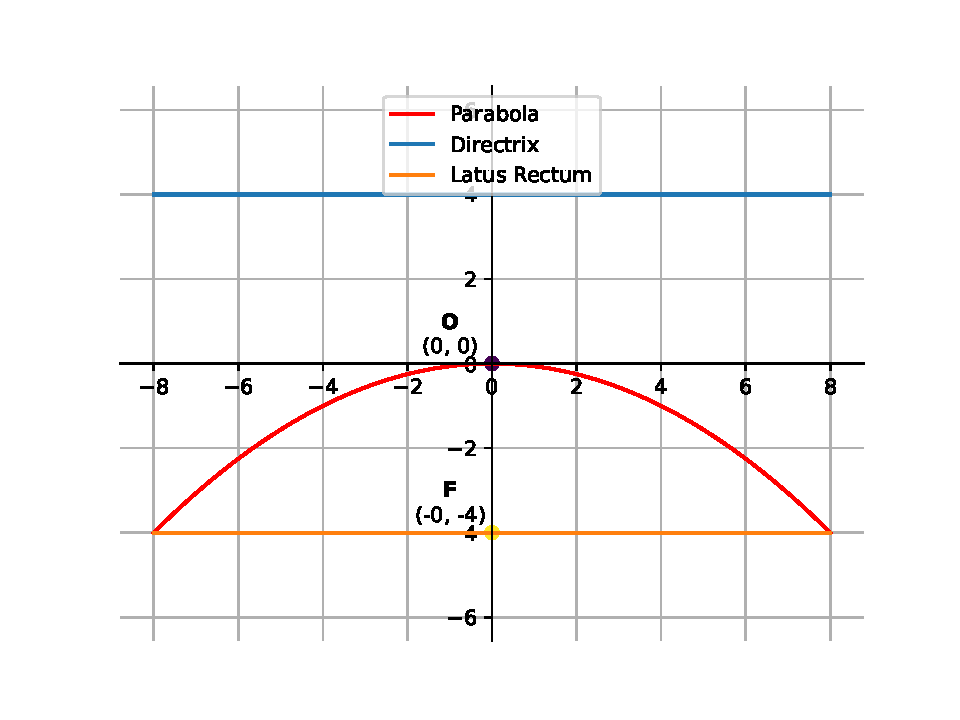
\includegraphics[width=0.75\columnwidth]{chapters/11/11/2/4/figs/fig.pdf}
	\end{center}
\caption{}
\label{fig:chapters/11/11/2/4/Fig1}
\end{figure}

\item 
$y^2 = –8x$
  \item $\frac{x^2}{36}+\frac{y^2}{16}=1$
\\
\solution
See 
\tabref{tab:std-conic-params-sol}
and 
\figref{fig:chapters/11/11/3/1/Fig1}.
\begin{figure}[H]
	\begin{center}
		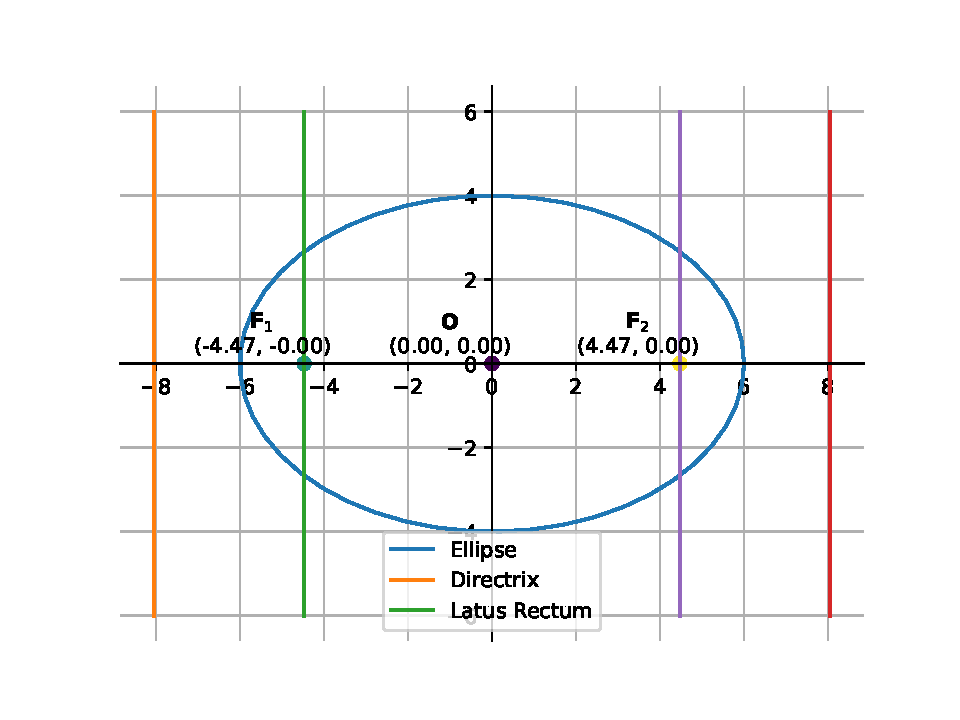
\includegraphics[width=0.75\columnwidth]{chapters/11/11/3/1/figs/fig.pdf}
	\end{center}
\caption{}
\label{fig:chapters/11/11/3/1/Fig1}
\end{figure}

  \item $\frac{x^2}{16}+\frac{y^2}{9}=1$
	\item $\frac{x^2}{16}-\frac{y^2}{9} = 1$. \\ 
		\solution
		See 
\tabref{tab:std-conic-params-sol}
and
\figref{fig:11/11/4/1Fig1}.
\begin{figure}[H]
	\begin{center}
		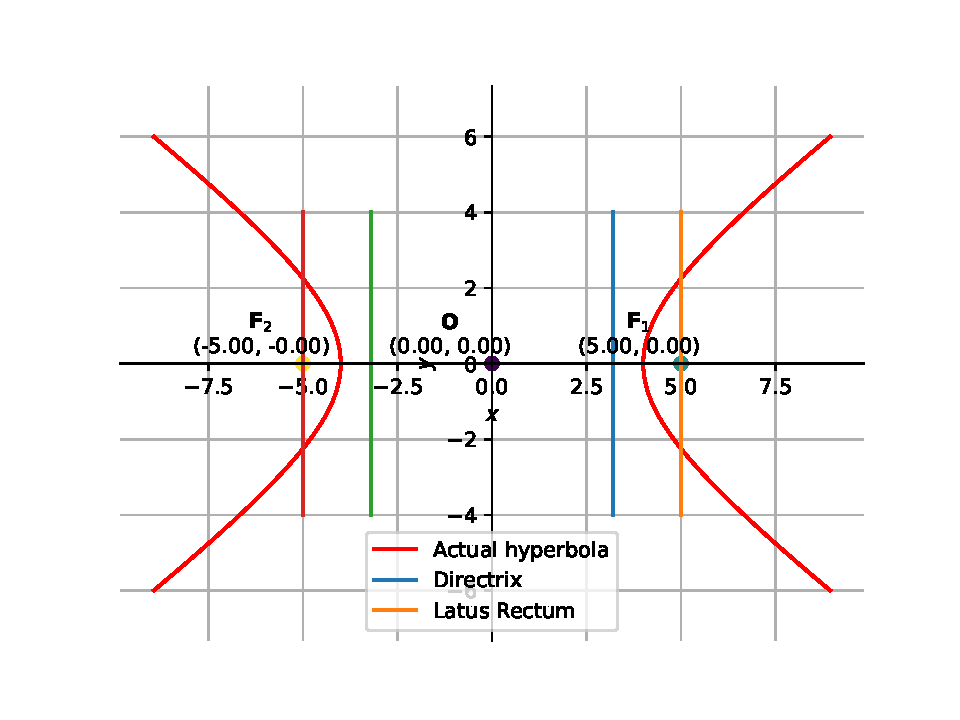
\includegraphics[width=0.75\columnwidth]{chapters/11/11/4/1/figs/fig.pdf}
	\end{center}
\caption{}
\label{fig:11/11/4/1Fig1}
\end{figure}

\begin{table}[H]
\centering
\caption{}
\label{tab:std-conic-params-sol}
\resizebox{\columnwidth}{!}{%
		\begin{tabular}{|c|c|c|c|c|c|c|}
\hline
\multicolumn{4}{|c|}{Input} & \multicolumn{3}{|c|}{Output} \\
\hline
Conic & $\vec{V}$ & $\vec{u}$ & $f$ & $\vec{F}$ & Directrix & Latus Rectum\\
\hline
$y^2=12x$  & $\myvec{0 & 0 \\ 0 & 1}$  & $-6\vec{e}_1$ & 0 & $3\vec{e}_1$ & $\vec{e}_1^{\top}\vec{x} = -3$ & 12 \\
\hline
$y^2=-8x$ &  $\myvec{0 & 0 \\ 0 & 1}$& $4\vec{e}_1$ & 0 & $-2\vec{e}_1$ & $\vec{e}_1^{\top}\vec{x} = 2$ & 8 \\
\hline
$\frac{x^2}{36}+\frac{y^2}{16}=1$ &\myvec{4&0\\0&9} & $\vec{0}$ &  -144& $2\sqrt{5}\vec{e}_1$ & $\vec{e}_1^{\top}\vec{x} = \frac{18}{\sqrt{5}}$ & $\frac{16}{3}$ \\
\hline
$\frac{x^2}{16}+\frac{y^2}{9}=1$ & $\myvec{9&0\\0&16}$ &$\vec{0}$    &  $-144$& $\pm\sqrt{7}\vec{e}_1$ & $\vec{e}_1^{\top}\vec{x} = \frac{16}{\sqrt{7}}$ & $\frac{9}{2}$ \\
\hline
$\frac{x^2}{16}-\frac{y^2}{9} = 1$ & $\myvec{ 9 & 0 \\ 0 & -16}$    & $\vec{0}$ & -144  & $\pm 5\vec{e}_1$ & $\vec{e}_1^{\top}\vec{x} = \frac{16}{5}$ & $\frac{9}{2}$ \\
\hline
\end{tabular}

		}
\end{table}
  \item $\frac{x^2}{4}+\frac{y^2}{25}=1$
\\
\solution
From \tabref{tab:rot-conic-params-sol}, it can be seen that this is not a standard ellipse, since $\lambda_1 > \lambda_2$.  Hence $\vec{P}$ plays a role and we need to use the affine transformation
\begin{align}
\vec{x} = \vec{P}\vec{y}
\end{align}
So the value of $\lambda_1$ and $\lambda_2$ need to be interchanged for all calculations and 
in
					\eqref{eq:dx-ell-hyp},
					$\vec{e}_2$ becomes the normal vector.
See \figref{fig:chapters/11/11/3/2/Fig1}.
\begin{figure}[H]
	\begin{center} 
	    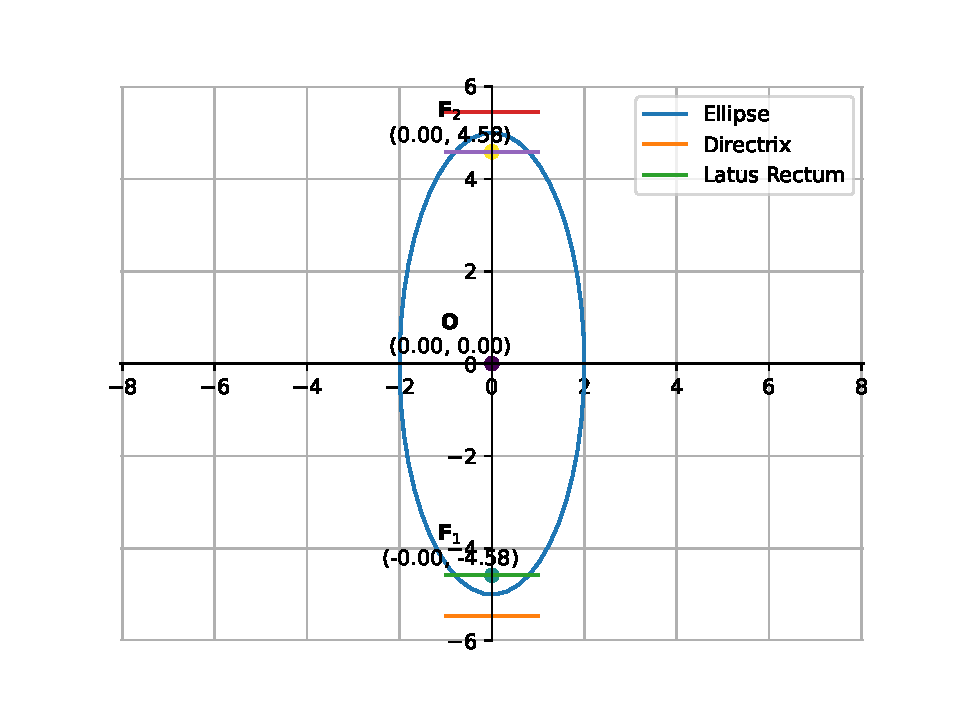
\includegraphics[width=0.75\columnwidth]{chapters/11/11/3/2/figs/fig.pdf}
	\end{center}
\caption{}
\label{fig:chapters/11/11/3/2/Fig1}
\end{figure}

	\item $5{y^2}-9{x^2}=36$.
		\\
		\solution
		\\
		See \tabref{tab:rot-conic-params-sol}
and 
\figref{fig:chapters/11/11/4/5/1}.
In
\tabref{tab:rot-conic-params-sol}, $\vec{P}$ shifts the negative eigenvalue 
to get the hyperbola in standard form.
\begin{figure}[H]
	\begin{center} 
	    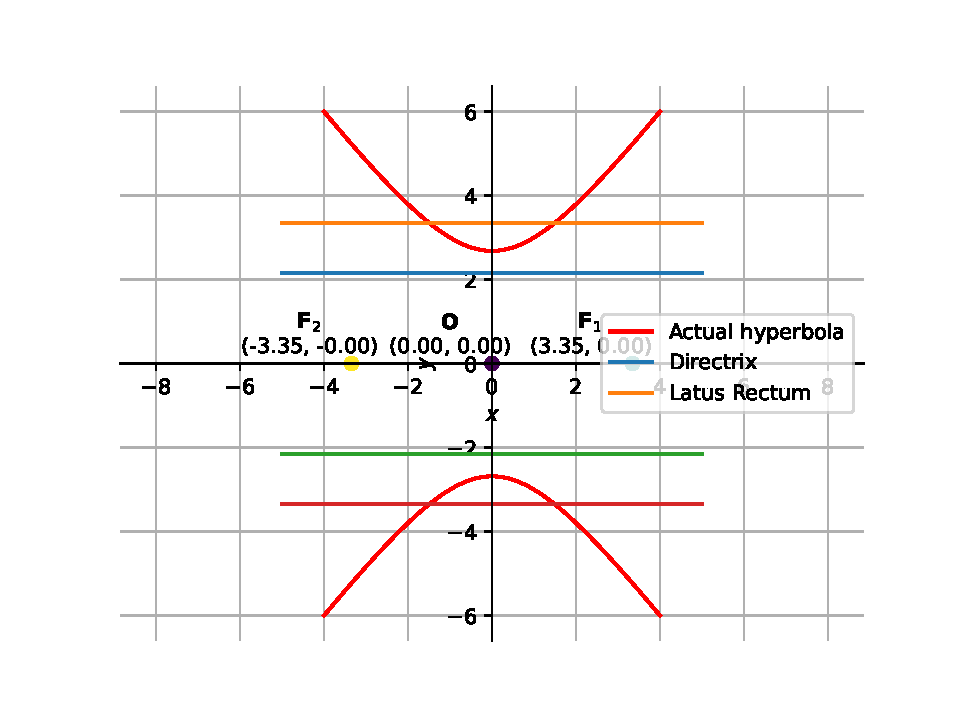
\includegraphics[width=0.75\columnwidth]{chapters/11/11/4/5/figs/fig.pdf}
	\end{center}
\caption{}
\label{fig:chapters/11/11/4/5/1}
\end{figure}


	\item $\frac{y^2}{9}-\frac{x^2}{27}=1$.
\item $x^2=-16y$
\\
\solution
See \tabref{tab:rot-conic-params-sol}
and 
\figref{fig:chapters/11/11/2/4/Fig1}.
\begin{figure}[H]
	\begin{center} 
	    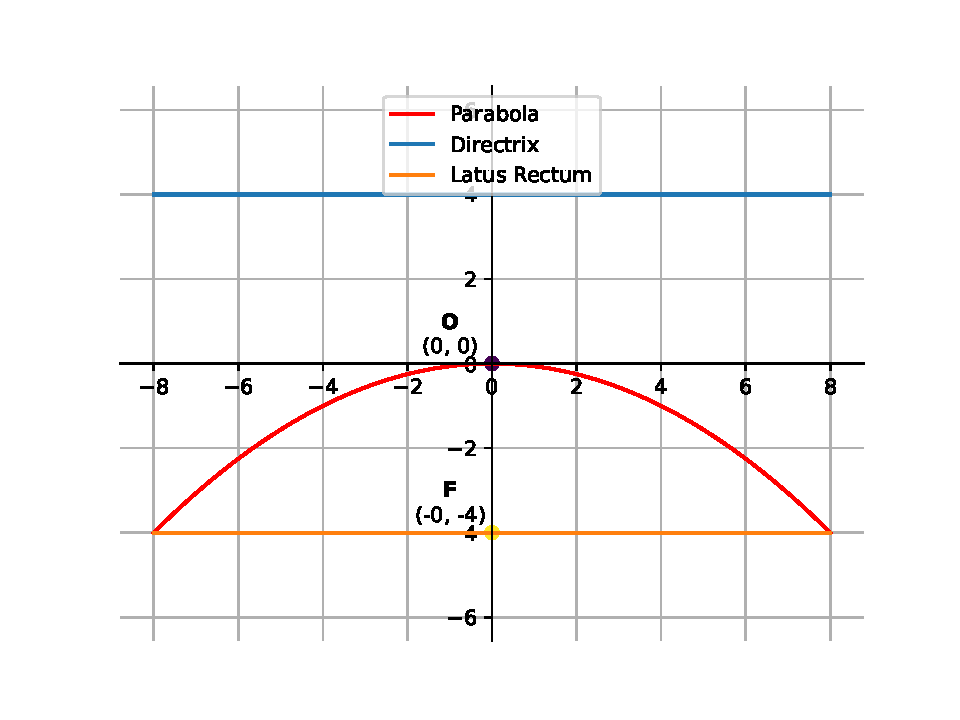
\includegraphics[width=0.75\columnwidth]{chapters/11/11/2/4/figs/fig.pdf}
	\end{center}
\caption{}
\label{fig:chapters/11/11/2/4/Fig1}
\end{figure}

\item $x^2=6y$ 
\begin{table}[H]
\centering
\caption{}
\label{tab:rot-conic-params-sol}
\resizebox{\columnwidth}{!}{%
		\input{chapters/conics/tables/rot.tex}
		}
\end{table}
\item $x^2=-9y$  
  \item $\frac{x^2}{25}+\frac{y^2}{100}=1$
  \item $\frac{x^2}{49}+\frac{y^2}{36}=1$
  \item $\frac{x^2}{100}+\frac{y^2}{400}=1$
  \item $36x^2+4y^2=144$
  \item $16x^2+y^2=16$
  \item $4x^2+9y^2=36$
\item $y^2=10x$  
\end{enumerate}

In each of the following exercises, find the equation of the conic, that satisfies the given conditions.

\begin{enumerate}[label=\thesubsection.\arabic*,ref=\thesubsection.\theenumi,resume*]
\item  foci \brak{\pm 4, 0}, latus rectum of length 12.
\\
\solution
		The given information is available in 
\tabref{tab:chapters/11/11/4/13/1}.
Since two foci are given, the conic cannot be a parabola.
\begin{enumerate}
\item The direction vector of $F_1F_2$ is the normal vector of the directrix.  Hence, 
\begin{align}
\vec{n} = \vec{F_1} - \vec{F_2}
	\equiv \vec{e}_1
\end{align}
Substituting in 
  \eqref{eq:conic_quad_form_v},
\eqref{eq:conic_quad_form_u}
and
\eqref{eq:conic_quad_form_f},
\begin{align}
	\vec{V} &= \myvec{1-e^2&0\\0&1} \label{eq:chapters/11/11/4/13/6} 
	\\
	\vec{u} &= ce^2\vec{e}_1-\vec{F}
\label{eq:chapters/11/11/4/13/6/u} 
	\\
	f&=16-c^2e^2
\label{eq:chapters/11/11/4/13/6/f} 
\end{align}
\item From
\eqref{eq:chapters/11/11/4/13/6},
\begin{align}
\lambda_1 &= 1-e^2,\
\lambda_2 = 1
\label{eq:chapters/11/11/4/13/12}
\end{align}
which upon substituting
in
			\eqref{eq:latus-ellipse}, along with the value of the latus rectum 
from \tabref{tab:chapters/11/11/4/13/1}
		\begin{align}
	6\brak{1-e^2} = \sqrt{\abs{f}}
\label{eq:chapters/11/11/4/13/12/f}
\end{align}
\item  The centre of the conic is given by
\begin{align}
\vec{c} = \frac{\vec{F_1} + \vec{F_2}}{2}
= \vec{0}
\label{eq:chapters/11/11/4/13/5}
\end{align}
From \eqref{eq:chapters/11/11/4/13/6}, it is obvious that  
$\vec{V}$ is invertible.  Hence,  
from \eqref{eq:chapters/11/11/4/13/5}
and 
\eqref{eq:conic_parmas_c_def},
\begin{align}
\vec{u} = \vec{0}
	\label{eq:chapters/11/11/4/13/7/u}
\end{align}
Substituting the above in \eqref{eq:chapters/11/11/4/13/6/u}, 
\begin{align}
\vec{F} = ce^2\vec{e}_1 
\implies 
	\norm{\vec{F}} = 4 = ce^2
	\label{eq:chapters/11/11/4/13/7}
\end{align}
\item 
	From 
      \eqref{eq:f0}, 
	\eqref{eq:chapters/11/11/4/13/7/u}
and
\eqref{eq:chapters/11/11/4/13/6/f},
		\begin{align}
	36\brak{1-e^2}^2 = 16-c^2e^2
\label{eq:chapters/11/11/4/13/12/ec}
\end{align}
From
	\eqref{eq:chapters/11/11/4/13/7}
	and
\eqref{eq:chapters/11/11/4/13/12/ec}
\begin{align}
\frac{4}{e\sqrt{e^2-1}} &= 6
\\
\implies 9e^2\brak{e^2-1} &= 4\\
\implies 9e^4-9e^2-4 &= 0
\\
	\text{or, }\brak{3e^2-4}
	\brak{12e^2+1} &=0
\label{eq:chapters/11/11/4/13/14}
\end{align}
yielding
\begin{align}
e = \frac{2}{\sqrt 3}
\end{align}
as the only viable solution.
\end{enumerate}
The equation of the conic is then obtained as
\begin{align}
\vec{x}^\top\myvec{-\frac{1}{3}&0\\0&1}\vec{x} +4 = 0
\end{align}
See \figref{fig:chapters/11/11/4/13/1}.
\begin{figure}[H]
\centering
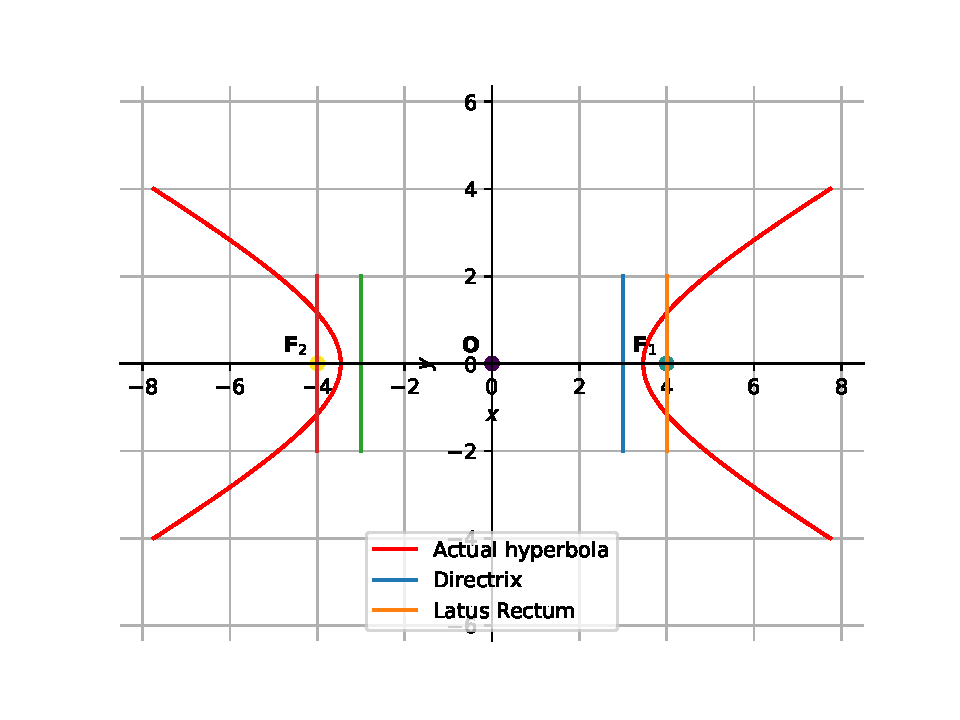
\includegraphics[width=0.75\columnwidth]{chapters/11/11/4/13/figs/fig.pdf}
\caption{}
\label{fig:chapters/11/11/4/13/1}
\end{figure}
\begin{table}[H]
\centering
\begin{tabular}[12pt]{ |c| c| c| c| }
\hline
$\beta$ & Airplane A & Airplane B & Airplane C \\
\hline
$\beta = -5\,\mathrm{deg}$ & $-0.030$ & $-0.025$ & $0.040$\\
\hline
$\beta = 0\,\mathrm{deg}$ & $0$ & $0$ & $0$ \\
\hline
$\beta = 5\,\mathrm{deg}$ & $0.030$ & $0.025$ & $-0.040$\\
\hline
\end{tabular}

\caption{}
\label{tab:chapters/11/11/4/13/1}
\end{table}

    \item eccentricity $e = \frac{4}{3}$,
    vertices 
    \begin{align}
        \vec{P_1} = \myvec{7\\0},\ \vec{P_2} = \myvec{-7\\0}
        \label{eq:chapters/11/11/4/14/vert}
    \end{align}
\\
\solution
		    The major axis of a conic is the chord which passes through the vertices of the conic.
    The direction vector of the major axis in this case is
    \begin{align}
        \vec{P}_2-\vec{P}_1 \equiv \vec{e}_1 = \vec{n}
\label{eq:chapters/11/11/4/13/6/n} 
    \end{align}
    which is the normal vector for the directrix.
    Since $e > 1$, the conic is a hyperbola.
Substituting  
\eqref{eq:chapters/11/11/4/13/6/n} 
in
  \eqref{eq:conic_quad_form_v},
\eqref{eq:conic_quad_form_u}
and
\eqref{eq:conic_quad_form_f},
\begin{align}
	\vec{V} = \myvec{1-e^2&0\\0&1} = \myvec{-\frac{7}{9}&0\\0&1} \label{eq:chapters/11/11/4/14/6} 
\end{align}
    The centre of the hyperbola is 
\begin{align}
	\vec{c} = \frac{\vec{P}_1+\vec{P}_2}{2} = \vec{0} = \vec{u}
\end{align}
from \eqref{eq:conic_parmas_c_def}.      Substituting $\vec{P}_1$ and $\vec{P}_2$ in 
    \eqref{eq:conic_quad_form},
    \begin{align}
        \vec{P}_1^\top\vec{VP}_1 + 2\vec{u}^\top\vec{P}_1 + f &= 0 \label{eq:chapters/11/11/4/14/ep1} \\
        \vec{P}_2^\top\vec{VP}_2 + 2\vec{u}^\top\vec{P}_2 + f &= 0 \label{eq:chapters/11/11/4/14/ep2}
	\\
	    \implies f = \vec{P}_1^\top\vec{VP}_1  = 49\brak{e^2-1}&=\frac{343}{9}
    \end{align}
    upon adding 
    \eqref{eq:chapters/11/11/4/14/ep2} and \eqref{eq:chapters/11/11/4/14/ep1}
    and simplifying.
    Therefore, the equation of the conic is
    \begin{align}
        \vec{x}^\top\myvec{-\frac{7}{9}&0\\0&1}\vec{x} + \frac{343}{9} = 0
    \end{align}
See \figref{fig:chapters/11/11/4/14/hyperbola}.
    \begin{figure}[H]
        \centering
        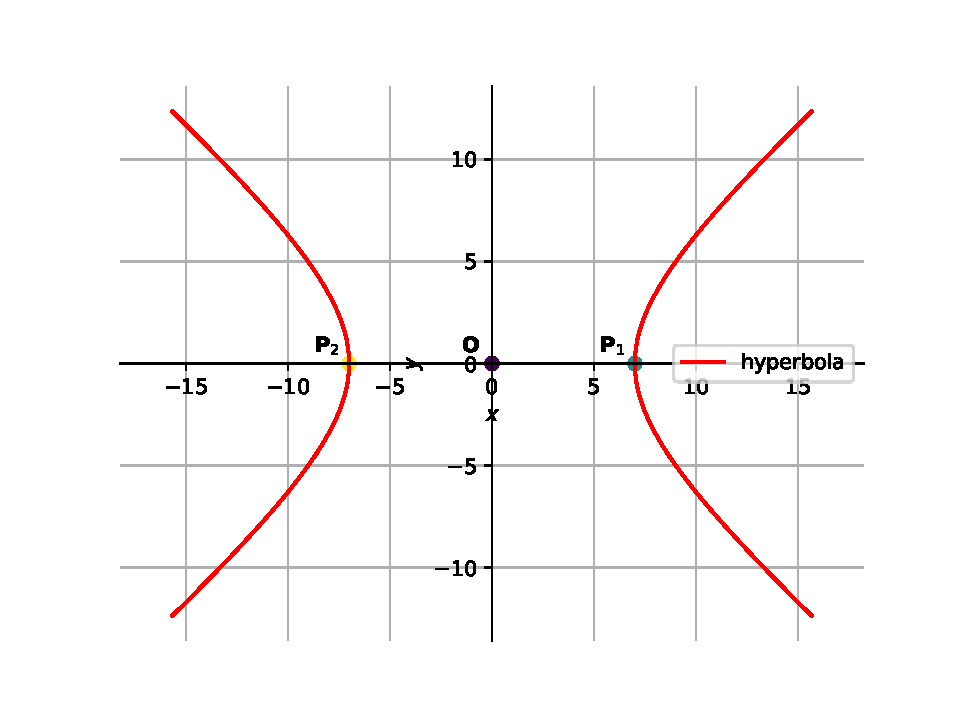
\includegraphics[width=0.75\columnwidth]{chapters/11/11/4/14/figs/fig.pdf}
        \caption{}
        \label{fig:chapters/11/11/4/14/hyperbola}
    \end{figure}

\item centre at $\vec{c}(0,0)$, major axis on the $Y$ axis and passes through the points $\vec{P}(3,2)$ and $\vec{Q}(1,6)$.
\\
\solution
Since the major axis is along the $y$-axis,
\begin{align}
\vec{n} = \vec{e}_2
\end{align}
Thus,
\begin{align}
\vec{V} = \myvec{1&0\\0&1-e^2} \label{eq:chapters/11/11/3/19/5} 
\end{align}
Since
\begin{align}
\vec{c} = \vec{0}, \vec{u}=\vec{0}.
\label{eq:chapters/11/11/3/19/8}
\end{align}
    From \eqref{eq:conic_quad_form},
    \begin{align}
        \vec{P}^\top\vec{VP} + 2\vec{u}^\top\vec{P} + f &= 0 \label{eq:chapters/11/11/3/19/ep1} \\
        \vec{Q}^\top\vec{VQ} + 2\vec{u}^\top\vec{Q} + f &= 0 \label{eq:chapters/11/11/3/19/ep2}
    \end{align}
    yielding
\begin{align}
4e^2 - f = 13 \label{eq:chapters/11/11/3/19/10}
\\
36e^2 - f = 37 \label{eq:chapters/11/11/3/19/11}
\end{align}
which can be formulated as the matrix equation
\begin{align}
\myvec{4&-1\\36&-1}\myvec{e^2\\f} = \myvec{13\\37}
\label{eq:chapters/11/11/3/19/12}
\end{align}
The augmented matrix is given by,
\begin{align*}
\myvec{4&-1&\vline&13\\36&-1&\vline&37}
\xleftrightarrow[]{R_1\leftarrow-\frac{R_1}{8}} \myvec{4&0&\vline&3\\36&-1&\vline&37} 
\\
\xleftrightarrow[]{R_2\leftarrow R_2-9R_1}
\myvec{4&0&\vline&3\\0&-1&\vline&10} 
\xleftrightarrow[R_2\leftarrow -R_2]{R_1\leftarrow \frac{R_1}{4}}
\myvec{1&0&\vline&\frac{3}{4}\\0&1&\vline&-10}
\end{align*}
Thus,
\begin{align}
e^2 = \frac{3}{4},\ f = -10
\end{align}
and the equation of the conic is given by
\begin{align}
\vec{x}^\top\myvec{1&0\\0&\frac{1}{4}}\vec{x} - 10 = 0
\end{align}
See  
\figref{fig:chapters/11/11/3/19/1}.
\begin{figure}[H]
\centering
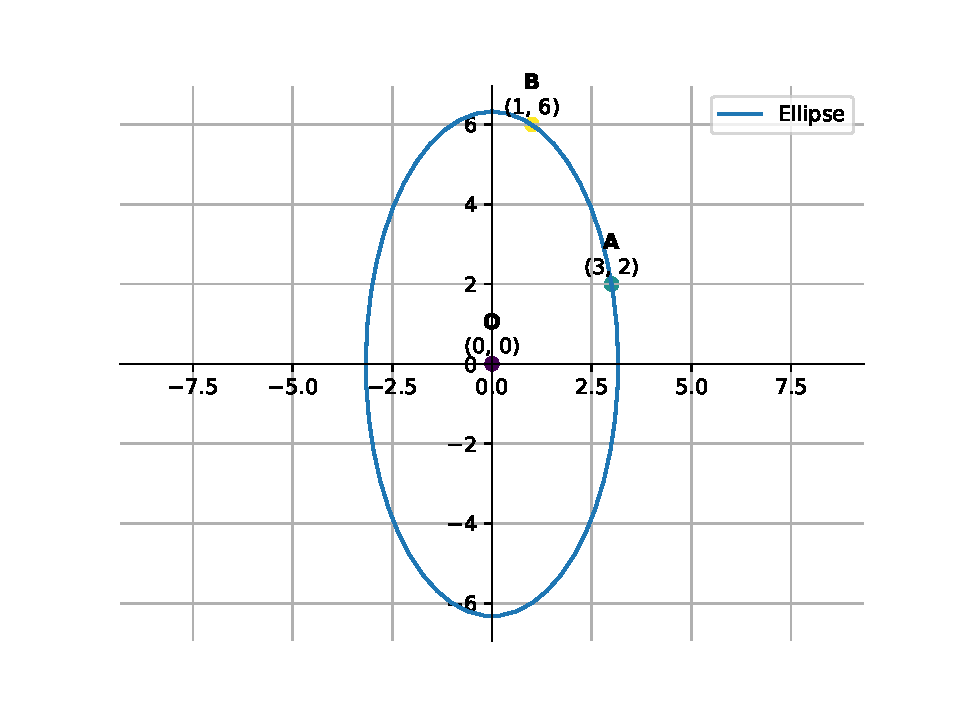
\includegraphics[width=0.75\columnwidth]{chapters/11/11/3/19/figs/fig.pdf}
\caption{}
\label{fig:chapters/11/11/3/19/1}
\end{figure}

\item major axis on the $X$ axis and passes through the points (4,3) and (6,2).
\\
\solution
In this case, 
    \begin{align}
        \vec{n} = \myvec{1\\0}
    \end{align}
    Thus,
    \begin{align}
        \vec{V} = \myvec{1-e^2&0\\0&1} \label{eq:chapters/11/11/3/20/V-val} \\
    \end{align}
Since
\begin{align}
\vec{c} = \vec{0}, \vec{u}=\vec{0}.
\label{eq:chapters/11/11/3/20/8}
    \end{align}
    From \eqref{eq:conic_quad_form},
    \begin{align}
        \vec{P}^\top\vec{VP} + 2\vec{u}^\top\vec{P} + f &= 0 \label{eq:chapters/11/11/3/20/ep1} \\
        \vec{Q}^\top\vec{VQ} + 2\vec{u}^\top\vec{Q} + f &= 0 \label{eq:chapters/11/11/3/20/ep2}
    \end{align}
    yielding
    \begin{align}
        16e^2 - f = 25 \label{eq:chapters/11/11/3/20/e1}
	\\
        36e^2 - f = 40 \label{eq:chapters/11/11/3/20/e2}
    \end{align}
which can be formulated as the matrix equation
    \begin{align}
        \myvec{16&-1\\36&-1}\myvec{e^2\\f} = \myvec{25\\40}
        \label{eq:chapters/11/11/3/20/mtx-eqn}
    \end{align}
    and can be solved using the augmented matrix.
    \begin{align*}
        \myvec{16&-1&25\\36&-1&40} \xleftrightarrow[]{R_1\leftarrow R_1-R_2} \myvec{-20&0&-15\\36&-1&40} \\
                 \xleftrightarrow[]{\substack{R_1\leftarrow\frac{R_1}{-5}\\R_2\leftarrow -R_2}} \myvec{4&0&3\\-36&1&-40} 
                 \xleftrightarrow[]{R_2\leftarrow R_2+9R_1}\myvec{4&0&3\\0&1&-13} \\
                 \xleftrightarrow[]{R_1\leftarrow\frac{R_1}{4}}\myvec{1&0&\frac{3}{4}\\0&1&-13}
    \end{align*}
    Thus,
    \begin{align}
        e^2 = \frac{3}{4},\ f = -13
    \end{align}
    and the equation of the conic is given by
    \begin{align}
        \vec{x}^\top\myvec{\frac{1}{4}&0\\0&1}\vec{x} - 13 = 0
    \end{align}
    See \figref{fig:chapters/11/11/3/20/ellipse}.
    \begin{figure}[H]
        \centering
        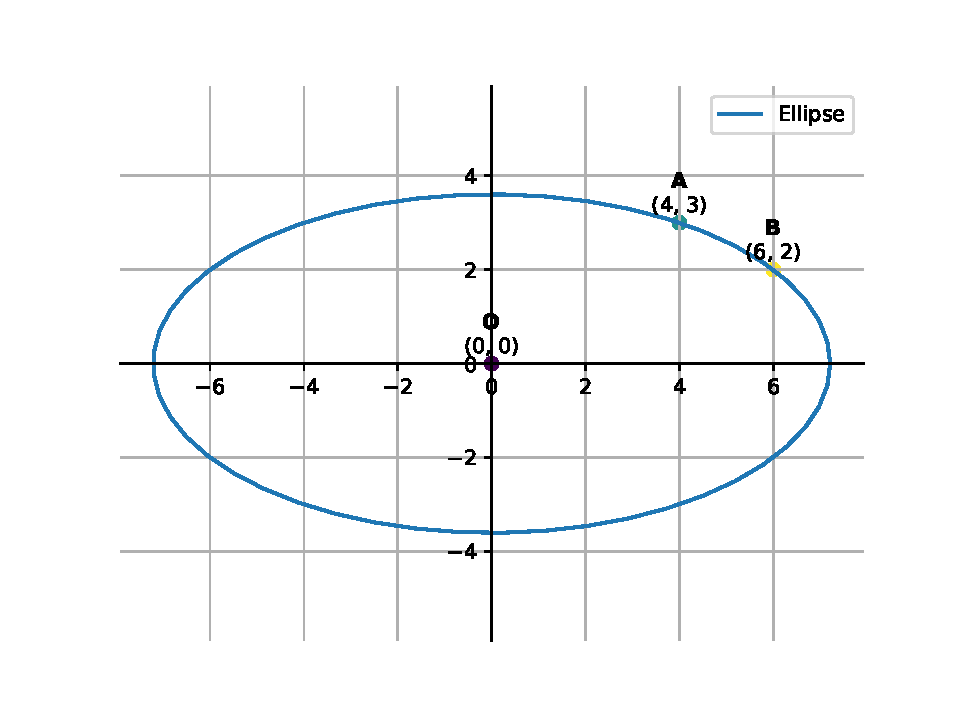
\includegraphics[width=0.75\columnwidth]{chapters/11/11/3/20/figs/fig.pdf}
        \caption{}
        \label{fig:chapters/11/11/3/20/ellipse}
    \end{figure}

\item vertices $\myvec{0\\\pm 3}$ and foci $\myvec{0\\\pm5}$.
	\\
\solution
		Following the approach in the earlier problems, it is obvious that
	\begin{align}
		\vec{n} 
			= \vec{e}_2,
	\vec{c} =\vec{u}=\vec{0}.
\end{align}
Consequently,
%
\begin{align}
	\vec{V} &= \myvec{1 &0\\ 0 & 1-e^2}
	\\
	\vec{F} &= ce^2\vec{e}_2 \implies \norm{\vec{F}} = ce^2=5
\label{eq:chapters/11/11/4/9/F}
	\\
	f 
	  &= 25 - c^2 e^2
\label{eq:chapters/11/11/4/9/f}
\end{align}
%
Since the vertices are  on the conic,
\begin{align}
	\vec{v_1}^{\top}\vec{V}\vec{v_1} +2\vec{u}^{\top}\vec{v_1}+f &= 0\\
\implies 9\brak{1-e^2} + f &= 0\\
 \label{eq:chapters/11/11/4/9/1}
\end{align}
Solving \eqref{eq:chapters/11/11/4/9/1},
\eqref{eq:chapters/11/11/4/9/F}
and
\eqref{eq:chapters/11/11/4/9/f},
\begin{align}
	c = \frac{9}{5},\ 
	e = \frac{5}{3},
\end{align}
%
yielding
\begin{align}
	\vec{V} = \myvec{1&0\\0& -\frac{16}{9}} ,\
	\vec{u} = \myvec{0\\0},\
	f = 16.
\end{align}
%
Thus, the desired equation of the hyperbola is
\begin{align}
	\vec{x}^{\top} \myvec{1&0\\ 0 & -\frac{16}{9}} \vec{x} +16 =0
\end{align}
%
See
%
    \figref{fig:chapters/11/11/4/9/}.
\begin{figure}[H]
  \centering
    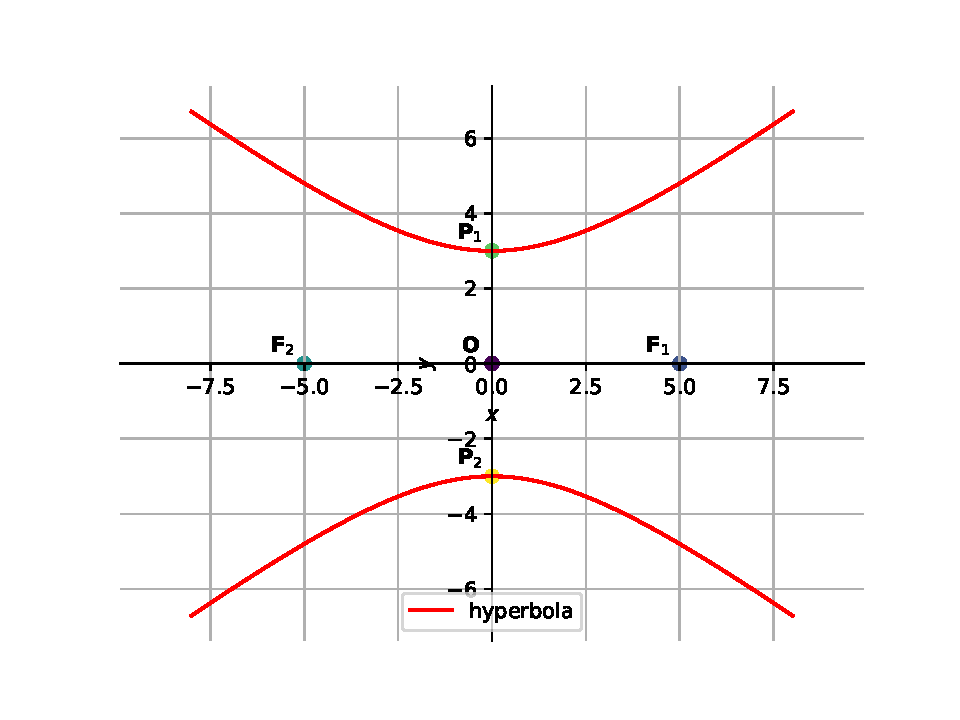
\includegraphics[width=0.75\columnwidth]{chapters/11/11/4/9/figs/fig.pdf}
    \caption{Figure 1}
    \label{fig:chapters/11/11/4/9/}
\end{figure}
%




\item vertices $\brak{0,\pm 5}, \text{foci} \brak{0,\pm 8}$.  
\item focus (6,0); directrix $x=-6$
\item focus $(0,-3)$; directrix $y=3$
\item vertex (0,0); focus (3,0)
\item vertex (0,0); focus $(-2,0) $
\item vertex (0,0) passing through (2,3) and axis is along $X$ axis
\item vertex (0,0) passing through (5,2) symmetric with respect to $Y$ axis
\item vertices $(\pm5,0),\text{foci} (\pm4,0)$.
\item vertices $(\pm0,13),\text{foci} (0,\pm5)$.
\item vertices $(\pm6,0),\text{foci} (\pm4,0)$.
\item ends of major axis $(\pm3,0)$, ends of minor axis $(0,\pm2)$.
\item ends of major axis $(0,\pm \sqrt{5})$, ends of minor axis $(\pm1,0)$.
\item length of major axis 26, foci $(\pm5,0)$.
\item length of minor axis 16, foci $(0,\pm6)$.
\item foci $(\pm3,0), a=4$.
\item vertex (0,4),  focus (0,2). 
\item vertex $(-3,0)$,  directrix $x+5=0$.
\item focus $(0,-3)$ and directrix $y=3$.
\item  directrix $x=0$, focus at (6,0).
\item  vertex  at (0,4), focus at (0,2).
\item  focus at $(-1,2)$, directrix $x-2y+3=0$.
	 \item  vertices $(\pm5,0)$, foci $(\pm 7,0)$.
	 \item vertices $(0\pm7), e =\frac{4}{3}$. 
	 \item  foci (0,$\pm\sqrt{10})$, passing through (2,3).
\item vertices at $(0,\pm6)$,  eccentricity $\frac{5}{3}$.
\item focus $(-1,-2)$,  directrix $x-2y+3=0$.
\item eccentricity $\frac{3}{2}$, foci $(\pm2,0)$.
 \item eccentricity $\frac{2}{3}$, latus rectum 5, centre  (0,0).
\item If the parabola $y^2=4ax$ passes through the point (3,2), then the length of its latus rectum is \rule{1cm}{0.1pt}.
\item Find the eccentricity of the hyperbola $9y^2-4x^2=36$.
\item Equation of the hyperbola with eccentricty $\frac{3}{2}$ and foci at ($\pm2,0)$ is \rule{1cm}{0.1pt}.
 \item Given the ellipse with equation $9x^2+25y^2=225,$ find the eccentricity and foci.
 \item Find the equation of the set of all points whose distance from (0,4) is $\frac{2}{3}$ of their distance from the line $y=9$.
\item The equation of the ellipse whose focus is $(1,-1)$, directrix $x-y-3
	=0$ and eccentricity $\frac{1}{2}$ is \rule{1cm}{0.1pt}.
\item The length of the latus rectum of the ellipse $3x^2+y^2=12$ is \rule{1cm}{0.1pt}.
\end{enumerate}
